\documentclass[tikz,dvisvgm]{standalone}
\usetikzlibrary{decorations.markings}
\usetikzlibrary{decorations.text}
\begin{document}
	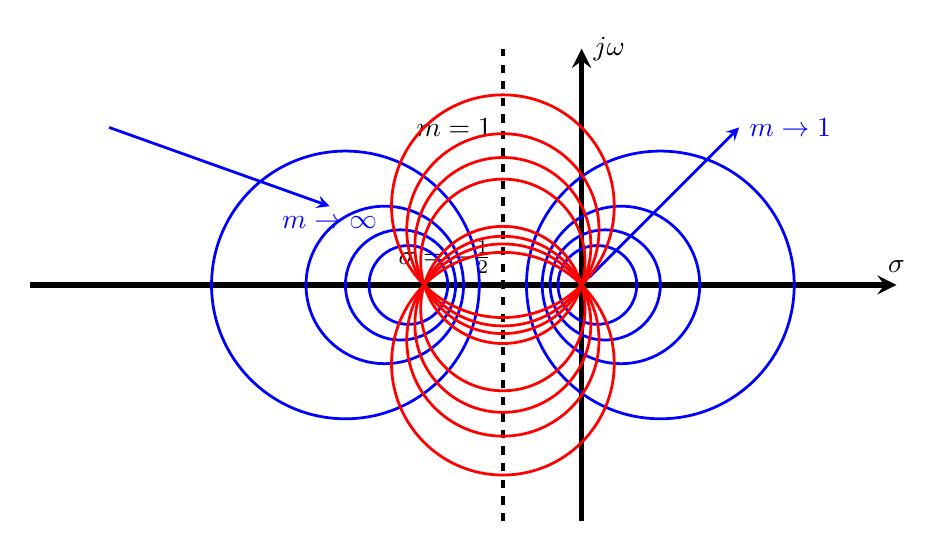
\begin{tikzpicture}
		% X and Y Axis
		\draw[line width=2pt, -stealth] (-7, 0) -- (4, 0) node[above] {$\sigma$};
		\draw[line width=2pt, -stealth] (0, -3) -- (0, 3) node[right] {$j\omega$};
		
		\def\axis{-1}
		
		\draw[line width=1.5pt, dashed] (\axis, -3) -- (\axis, 0) node [above left] {$\sigma = -\frac{1}{2}$} -- (\axis, 2) node[left] {$m=1$} -- (\axis, 3);
		
		% Isogain
		\draw[blue, line width=1pt] (\axis + 1 + 0.2, 0) circle[radius=0.5];
		\draw[blue, line width=1pt] (\axis + 1 + 0.3, 0) circle[radius=0.7];
		\draw[blue, line width=1pt] (\axis + 1 + 0.5, 0) circle[radius=1.0];
		\draw[blue, line width=1pt] (\axis + 1 + 1.0, 0) circle[radius=1.7];
		
		\draw[blue, line width=1pt] (\axis - 1 - 0.2, 0) circle[radius=0.5];
		\draw[blue, line width=1pt] (\axis - 1 - 0.3, 0) circle[radius=0.7];
		\draw[blue, line width=1pt] (\axis - 1 - 0.5, 0) circle[radius=1.0];
		\draw[blue, line width=1pt] (\axis - 1 - 1.0, 0) circle[radius=1.7];
		
		\draw[blue, line width=1pt, -stealth] (0.1, 0.1) -- (2, 2) node[blue, right] {$m \to 1$};
		\draw[blue, line width=1pt, -stealth] (-6, 2) -- (-3.2, 1) node[blue, below] {$m \to \infty$};
		
		% Isophase
		\begin{scope}[red, line width=1pt]
			\foreach \y in {-1, -0.7, -0.5, -0.3, 0.3, 0.5, 0.7, 1}
			\draw (\axis, \y) circle[radius={sqrt(\axis*\axis + \y*\y)}];
		\end{scope}
	\end{tikzpicture}
\end{document}
